\section{Versuchsaufbau}
%skizze zum versuchsaufbau (oder foto) einf�gen,   es muss erkl�rt werden wie das ganze funktioniert und welche speziellen einstellungen verwendet wurden (z.b. welche kn�pfe an den ger�ten f�r die messung verdreht wurden)


Der Versuchsaufbau besteht Haupts�chlich aus einem Laser, einem Polarisationsdreher, einer Sammellinse, zwei Rotationstischen mit Justiereinheit, Probenhalterung und einem Detektor. 

Der Laser, der Polarisationsdreher und die Sammellinse sind auf einer optischen Bank befestigt. Bei dem Laser handelt es sich um einen Diodenlaser der Klasse II, mit einer Wellenl�nge von 670 nm $\pm$ 10 nm, die Ausgangsleistung ist kleiner als 1mW. Der Strahl hat einen Durchmesser von 3mm und eine Divergenz von weniger als 0.5mrad \cite{Versuchsanleitung}. Mit dem Polarisationsdreher kann die Polarisationsrichtung des Laserstrahl mit einer Pr�zision von 0.5$^\circ$ beliebig eingestellt werden \cite{Versuchsanleitung}. Die erste Sammellinse dient dazu, die Laserstrahl auf die Probenoberfl�che zu fokussieren und hat eine Brennweite von 100mm \cite{Versuchsanleitung}. Durch weitere Sammellinsen mit den Brennweiten von 150mm, 200mm und 250mm kann der Laserstrahl noch auf den Detektor fokussiert werden \cite{Versuchsanleitung}.

Hinter der optischen Bank befindet sich die beiden Rotationstische mit Justiereinheit. Die beiden Rotationstische sind entkoppelt von einander auf einer Aluminiumplatte installiert. Mit dem oberem Rotationstisch kann der Einfallswinkel des Laserstrahls mit eine Genauigkeit von 0.02$^\circ$ bestimmt werden \cite{Versuchsanleitung}. Der Ausfallswinkel des reflektierten Strahls wird �quivalent mit dem unterem Rotationstische bestimmt. Auf den beiden Rotationstischen ist ein Lineartisch, mit zwei Goniometern und eine Probenhalterung installiert. �ber die beiden Goniometer l�sst sich die Oberfl�che der Probe in einem Bereich von $\pm 5^\circ$ justiert werden \cite{Versuchsanleitung}. Als Detektor wird eine Silizium-Photodiode, mit integriertem Messverst�rker verwendet. Das Signal wird mit einem Digitalmultimeter aufgenommen. Da die Silizium-Photodiode eine hohe Empfindlichkeit im gesamten Spektrum des sichtbaren Lichts hat, kann das Umgebungslicht mit einen Rotfilter ged�mpft werden, dabei wird das Licht von Gl�hlampen um ca. 50\% und das Licht von Leuchtstoffr�hren um ca. 10\% ged�mpft.

Die der Versuchsaufbau ist in Abb. \ref{fig:aufbau_1} und Abb. \ref{fig:aufbau_2} zu sehen.

\begin{figure}[H]
\centering
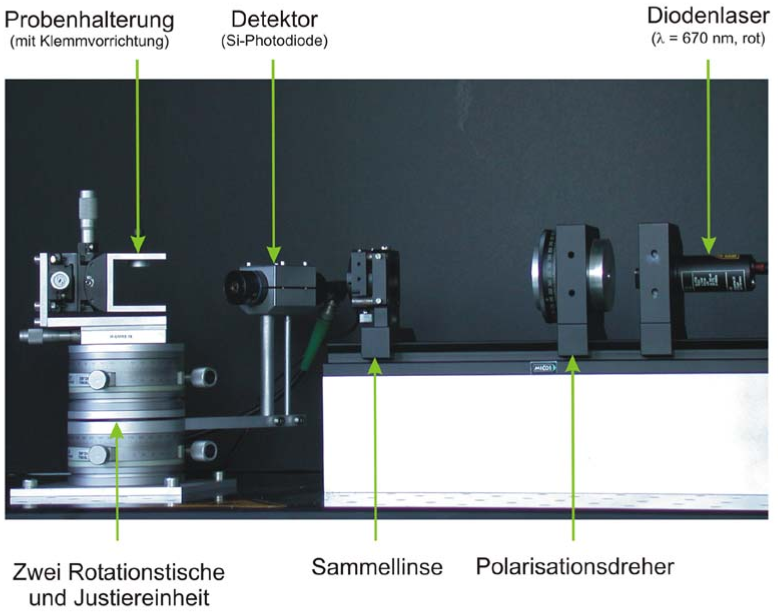
\includegraphics[scale = 0.39]{aufbau_1.png}
\caption{Gesamtaufbau der Messapparatur, entnommen von \cite{Versuchsanleitung}}
\label{fig:aufbau_1}
\end{figure}


\begin{figure}[H]
\centering
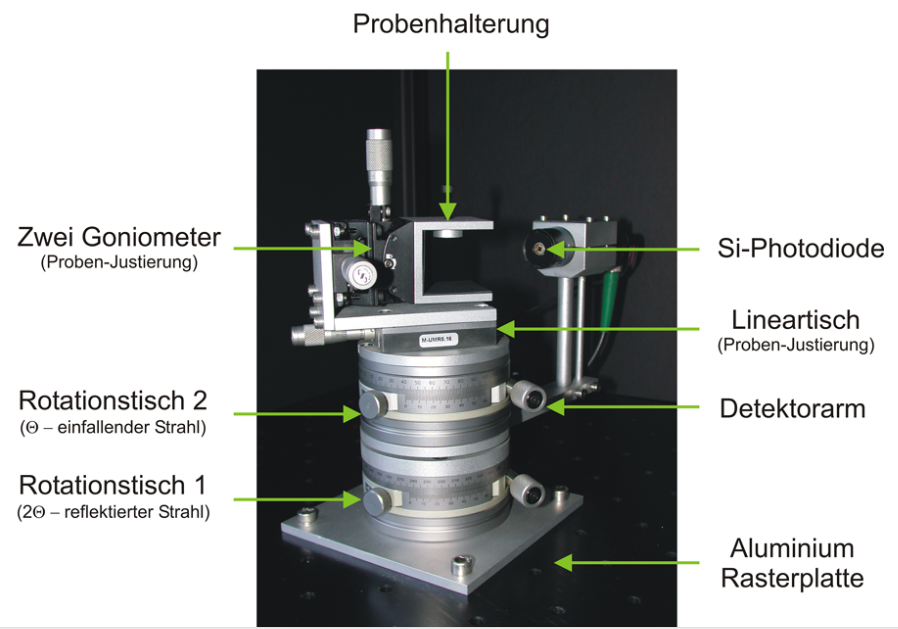
\includegraphics[scale = 0.39]{aufbau_2.png}
\caption{ Aufbau der Rotationstische und der Prismenhalterung, entnommen von \cite{Versuchsanleitung}}
\label{fig:aufbau_2}
\end{figure}


